\documentclass[11pt,a4paper,titlepage]{article}
\usepackage[utf8]{inputenc}
\usepackage[english]{babel}
\usepackage[T1]{fontenc}

\RequirePackage[layout=inline]{fixme}

\usepackage{float}
\usepackage{graphicx}
\usepackage{setspace}
\usepackage{amsmath}
\usepackage{courier}
\usepackage{amsmath}
\usepackage{listings}
\usepackage{color}
\usepackage[toc, page]{appendix}

\usepackage{algpseudocode}
\usepackage[bottom]{footmisc}
\usepackage{verbatimbox}

\usepackage{changepage}

\definecolor{mygreen}{rgb}{0,0.6,0}
\definecolor{mygray}{rgb}{0.5,0.5,0.5}
\definecolor{mymauve}{rgb}{0.58,0,0.82}


%% Units:
\newcommand{\mA}{\,\textrm{mA}}
\newcommand{\N}{\,\textrm{N}}
\newcommand{\Hz}{\,\textrm{Hz}}
\newcommand{\V}{\,\textrm{V}}
\newcommand{\Ohms}{\,\Omega}
\newcommand{\kOhm}{\,\text{k}\Omega}
\newcommand{\nF}{\,\textrm{nF}}
\newcommand{\dB}{\,\textrm{dB}}
\newcommand{\VperBit}{\,\textrm{V/bit}}
\newcommand{\NperBit}{\,\textrm{N/bit}}

\lstset{ %
	backgroundcolor=\color{white},   % choose the background color
	basicstyle=\scriptsize,        % size of fonts used for the code
	breaklines=true,                 % automatic line breaking only at whitespace
	captionpos=b,                    % sets the caption-position to bottom
	commentstyle=\color{mygreen},    % comment style
	escapeinside={\%*}{*)},          % if you want to add LaTeX within your code
	keywordstyle=\color{blue},       % keyword style
	stringstyle=\color{mymauve},     % string literal style
	numbers=left,
}

%\renewcommand{\thesubsection}{\thesection.\alph{subsection}}



\usepackage{booktabs}
\usepackage[backend=biber, bibencoding=utf8, style=ieee]{biblatex}

\addbibresource{references.bib}
\usepackage[final,hidelinks]{hyperref} % must be last package loaded

\author{Ólafur Jón Thoroddsen}  % My name, for the titlepage
\title{\includegraphics{graphics/ru-logo}\\\vspace{10mm}
	Mechatronics II\\T-535-MECH \ \\Homework 8}  % The title, for the titlepage

\begin{document}
	\pagenumbering{arabic}
	\maketitle
	
	\tableofcontents
	\pagebreak
	
	\section{A Weight Scale\label{sec:scale}}
	\subsection{Signal analysis}
	The signal coming from a weight scale ranges from $4-20\mA$ for $0-100\N$ of force. An ADC samples the signal at $300\Hz$ with a range of $0-3\V$ at 10bit resolution. A $5\mA, 1000\Hz$ noise is beside the signal coming from the scale. 
	
	To get rid of the noise, a filtering circuit is required that will attenuate the noise but keep the signal as clean as possible. From the ADC specifications, it is safe to assume that the signal is at a frequency below $150\Hz$, due to the Nyquist - Shannon sampling theorem. Thus, we can safely design our filtering circuit to have a 3dB frequency of $300\Hz$ and be sure not to lose any of the actual signal.
	
	
	\subsection{Filtering Circuit}
	A third order active low pass filter can be created by connecting three first order filters in a cascade as shown in figure~\ref{fig:cascadefilters}.
	
	\begin{figure}[h]
		\centering
		\includegraphics[width=\textwidth]{graphics/thirdorderlowpass}
		\caption{A third order low pass active filter with unity gain.}
		\label{fig:cascadefilters}
	\end{figure}
	%A simple unity gain 1st order active filter can be created by connecting a passive RC filter to a voltage follower as shown in figure~\ref{fig:lowpass}. With the components chosen as in the figure, the transfer function will be
	
	\noindent The transfer function of this circuit is given by multiplying together the transfer functions of each individual components.
	
	\begin{equation}
	\begin{aligned}
		\frac{\text{V}_{out}}{\text{V}_{in}} &= \frac{\text{V}_{out}}{\text{V}_2} \cdot \frac{\text{V}_2}{\text{V}_1} \cdot \frac{\text{V}_{1}}{\text{V}_{in}}\\
	\end{aligned}
	\end{equation}

	\noindent so
	\begin{equation}
	\begin{aligned}
		\frac{\text{V}_{out}}{\text{V}_{in}} &= \frac{1}{1 + s/\omega_1} \cdot \frac{1}{1 + s/\omega_2} \cdot \frac{1}{1 + s/\omega_3}\\
		 %&= \frac{1}{1 + s R_3 C_3} \cdot \frac{1}{1 + s R_2 C_2} \cdot \frac{1}{1 + s R_1 C_1}\\
		 \label{eq:transfer}
	\end{aligned}
	\end{equation}

	\noindent where 
	\[
	\begin{aligned}
		\omega_1 &= \frac{1}{R_1C_1}\\
		\omega_2 &= \frac{1}{R_2C_2}\\
		\omega_3 &= \frac{1}{R_3C_3}\\
	\end{aligned}
	\]
	 For this application, it is chosen to have all the 3dB frequencies the same. That way, the signal will be attenuated by -60dB/decade from 300\Hz.
	 
	 \noindent That is
	 
	 \[
	 \begin{aligned}
		 R = R_1 = R_2 = R_3\\
		 C = C_1 = C_2 = C_3\\
	 \end{aligned}
	 \]
	 
	 \noindent To obtain a 3dB frequency of approximately 300\Hz, capacitances $C_1$, $C_2$ and $C_3$ are chosen to be $C = 47\nF$ (because it commonly used and is available. Other capacitances could be used, the only thing affected would be the value of the resistance). The required value of the resistors is then 
	 
	 \[
	 \begin{aligned}
		 R &= \frac{1}{2\pi\times 300 \times 47\times 10^{-9}} = 11,28\kOhm \\
	\end{aligned}
	 \]
	
	\noindent A third order filter like this will have a frequency response with a slope of -60dB per decade after the 3dB frequency, which means that at $3000\Hz$ the input signal will be attenuated by 60dB. From equation~\ref{eq:transfer}, the noise at $1000\Hz$ and will be attenuated by 
	
	\[
	\begin{aligned}
		T(1000\times 2\pi) &= 0,0123\\
		&\approx -38,2\dB\\
	\end{aligned}
	\]
	\noindent So the largest amount of signal noise will be $5\mA \times 0,0123 \approx 0,0615\mA$ 
	
	\subsection{Extracting the signal}
	
	The signal is a current ranging from 4-20\mA which must be converted to a voltage to be able to put it through the filter and into the ADC. To convert the current, a resistor is connected from the filter input to ground.
	
	The ADCs range is 0-3\V, so to reach 3V with a 20\mA\ current, a resistance of $R = 3/0,020 = 150\Ohms$ is required. So for a 0\N\ force, a voltage of $0,004 \times 150 = 0,6\V$ will be outputted by the scale.
	The signal limits the voltage range of the ADC to $0,6 - 3\V$, which gives a resolution of 
	
	\begin{equation}
		\text{res} = \frac{3 - 0,6}{2^{10}} = 0,00234\VperBit
	\end{equation}
	
	\noindent or in Newtons
	\begin{equation}
		\text{res} = \frac{100}{2^{10}} = 0,00976\NperBit
	\end{equation}
	
	I have some bad feeling about these calculations. Because the signal is at minimum 0,6\V\, it is not possible to utilize the ADCs entire range so the resolution cannot be as high as stated above. At the moment this is written, time is not an expendable resource so this will be left for later scrutiny.
	
	
	\section{Types of filters}
	\subsection{Low pass filters}
	A low pass filter is a circuit or a mathematical function that only allows slowly changing signals to pass through. An example of a low pass filter circuit is the three stage filter in figure~\ref{fig:cascadefilters}.
	The frequency response of a first order low pass filter is shown in figure~\ref{fig:lowpass}. These types of filters are used widely, for example to cancel out high frequency noise as in section~\ref{sec:scale}.
	
	\begin{figure}[h]
		\centering
		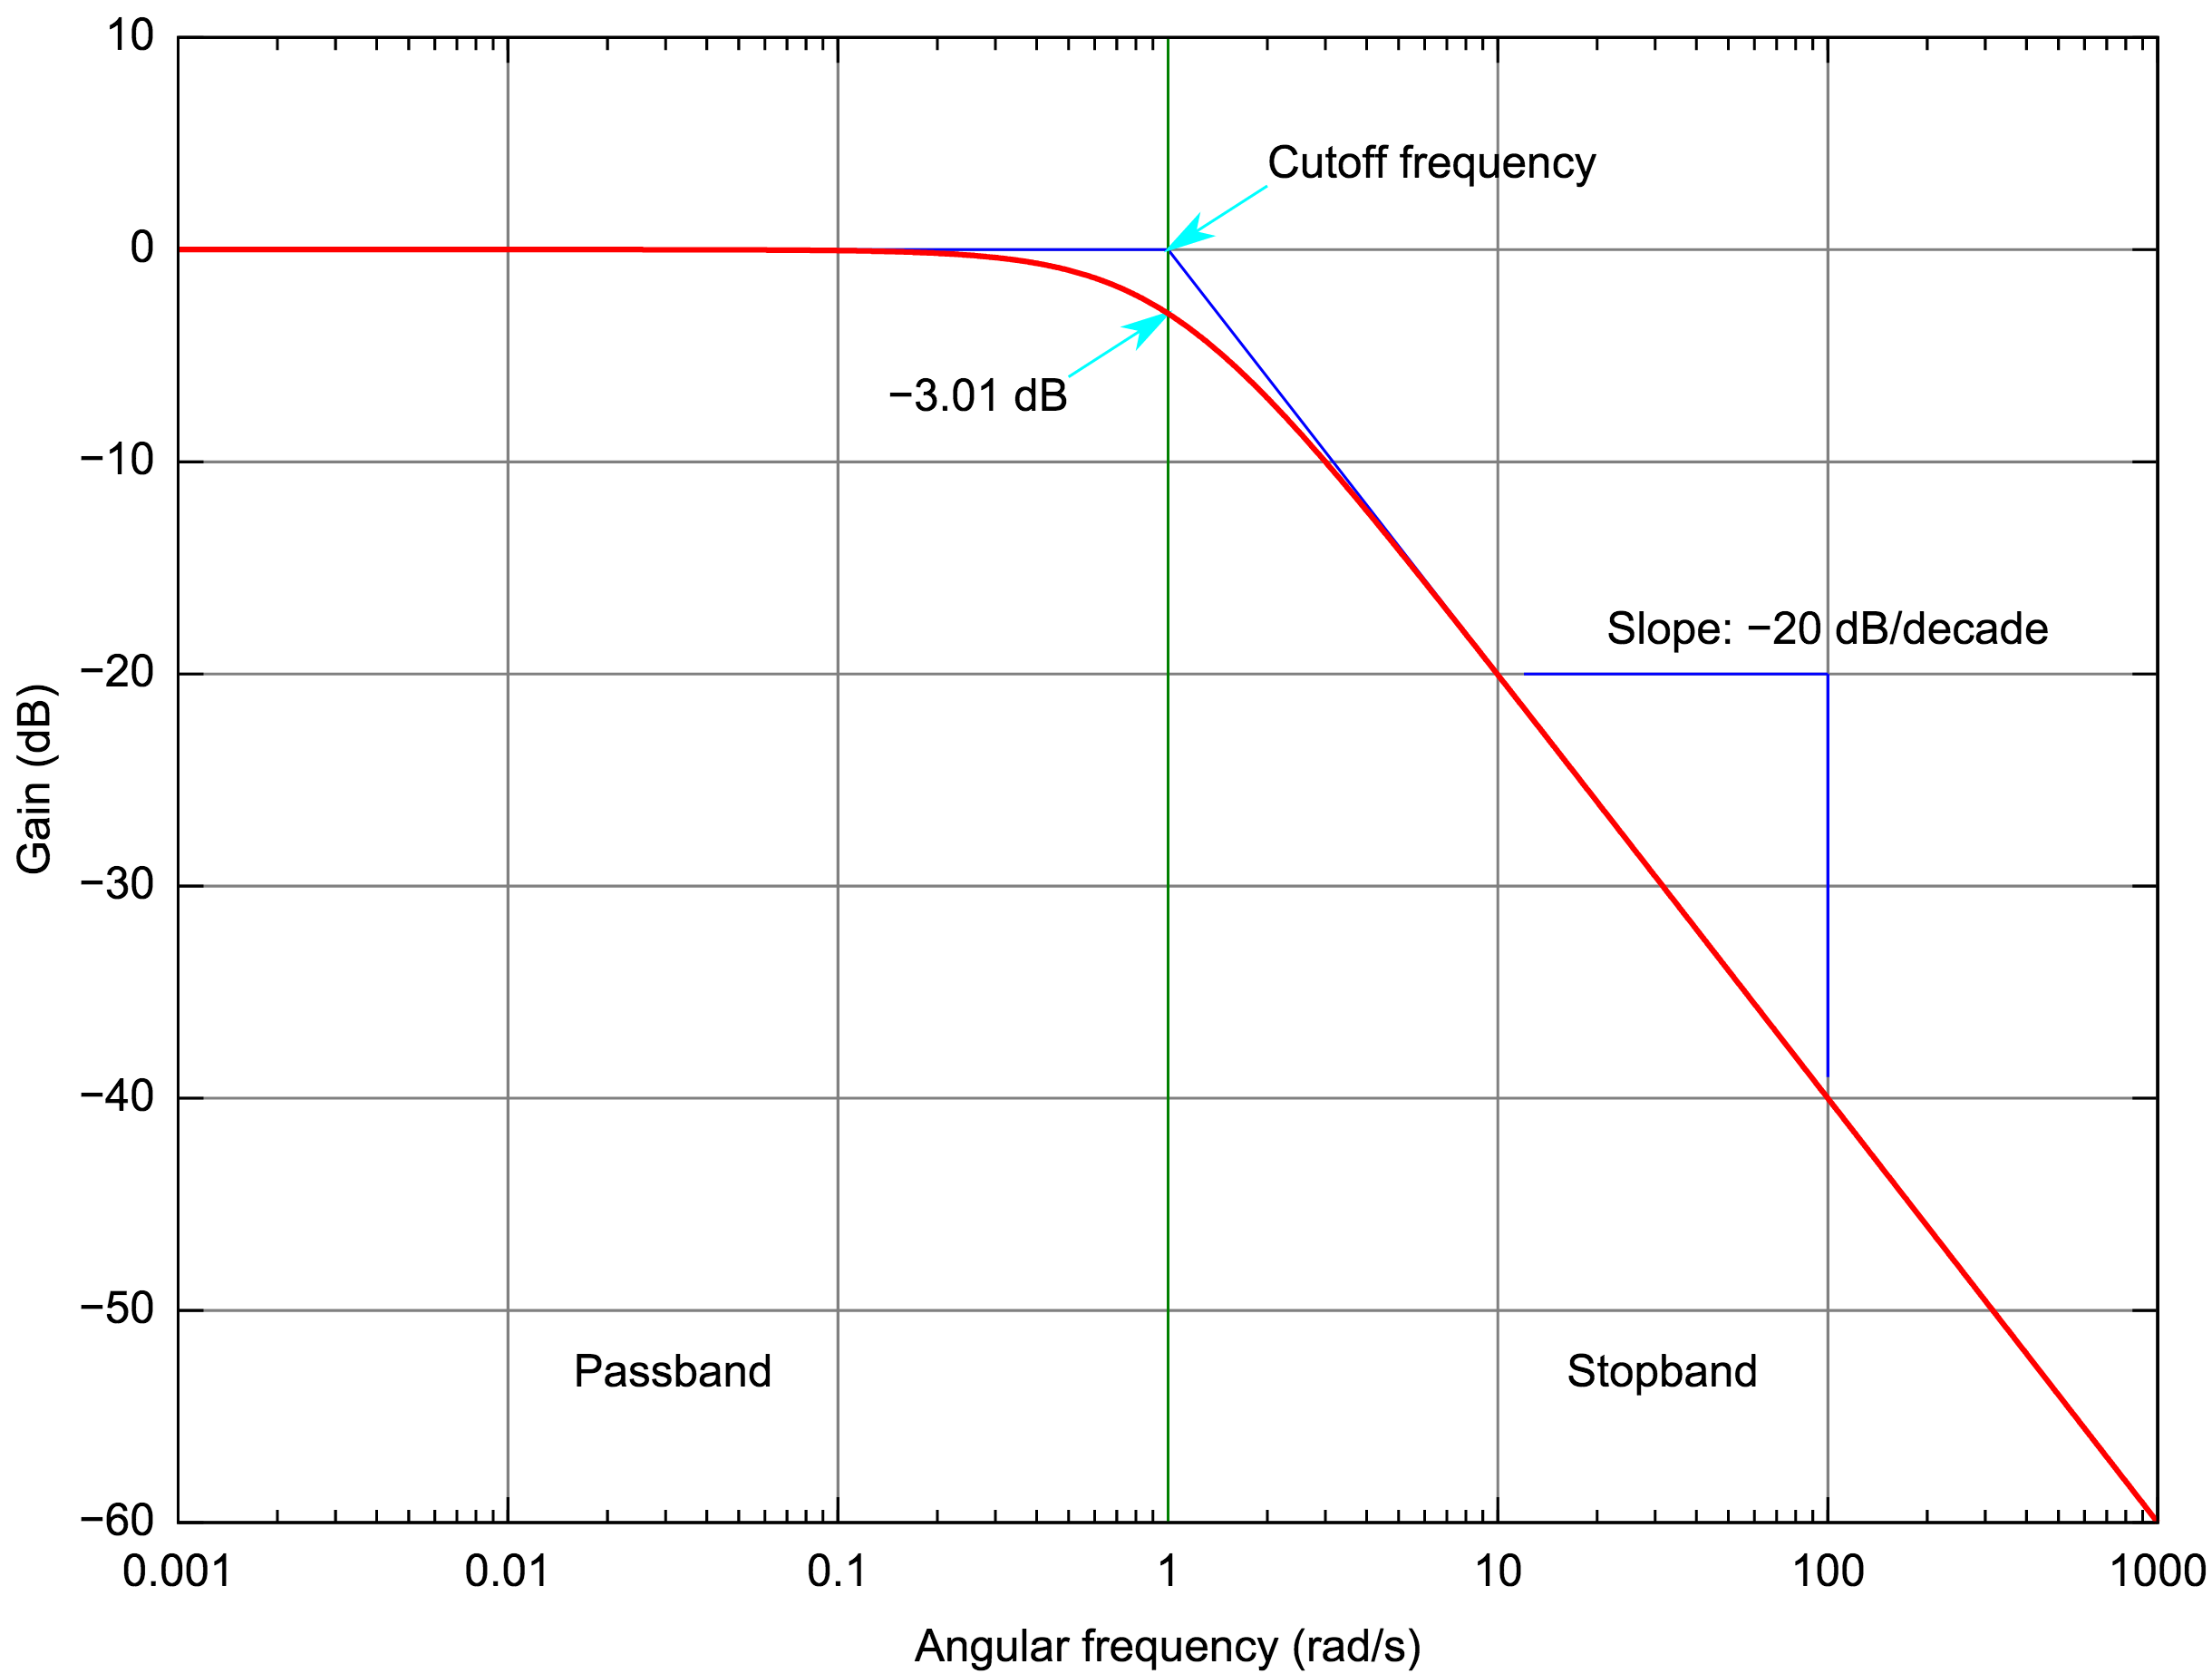
\includegraphics[width=0.6\textwidth]{graphics/lowpassbode}
		\caption{The frequency response of a first order low pass filter~\cite{lowpass}.}
		\label{fig:lowpass}
	\end{figure}
	
	
	\subsection{High pass filters}
	A high pass filter is a circuit or a mathematical function that only allows rapidly changing signals to pass through. The frequency response of those filters are similar to those as seen in figure~\ref{fig:highpass}.
	
	\begin{figure}[h]
		\centering
		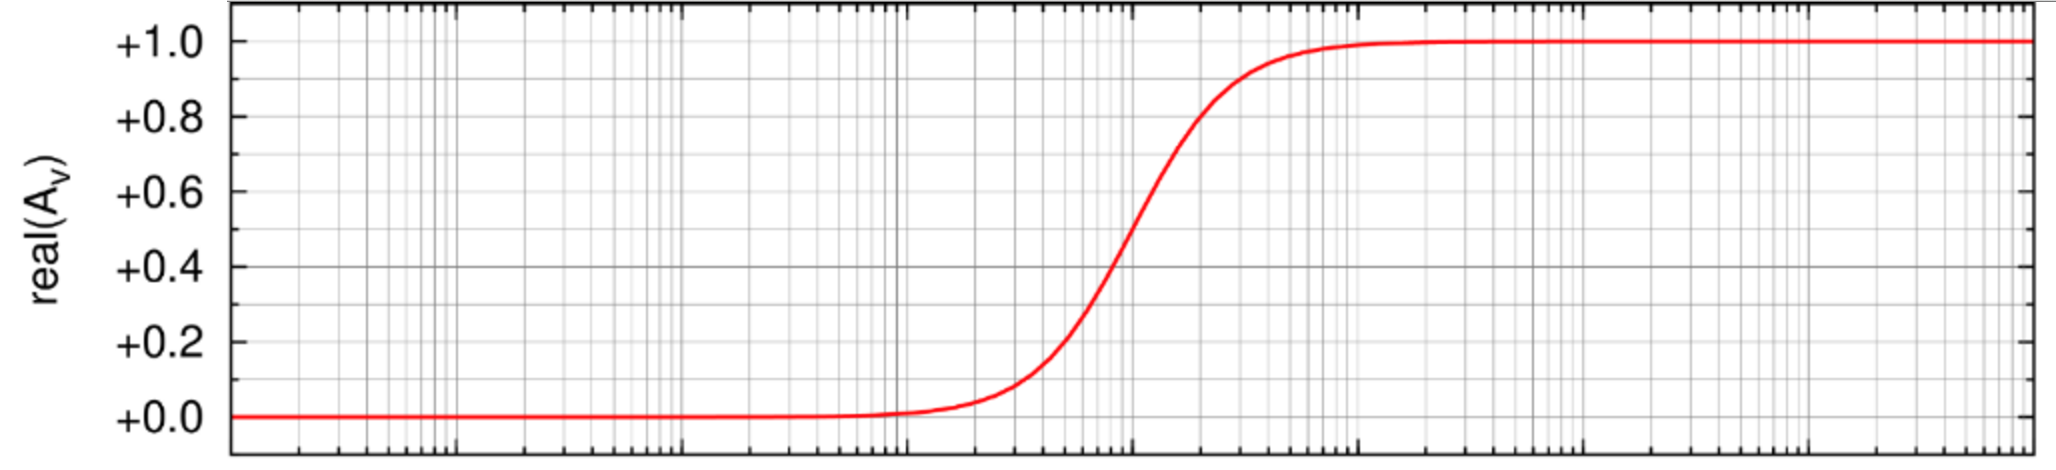
\includegraphics[width=\textwidth]{graphics/highpassbode}
		\caption{The frequency response of a high pass filter with some 3dB frequency $\omega_0$. The y axis in this figure is linear, yielding a gain of 1 at high frequencies~\cite{highpass}.}
		\label{fig:highpass}
	\end{figure}
	
	
	\subsection{Bandpass filters}
	A bandpass filter is a circuit or a mathematical function that only allows a certain spectrum of signals to pass through. Signals lower then some 3dB frequency $\omega_L$ will be attenuated, and signals higher then another 3dB frequency $\omega_H$ will also be attenuated. Signals with frequencies between $\omega_L$ and $\omega_H$ will be allowed to pass through.
	The frequency response of such a filter can be seen in figure~\ref{fig:bandpass}.
	
	\begin{figure}[h]
		\centering
		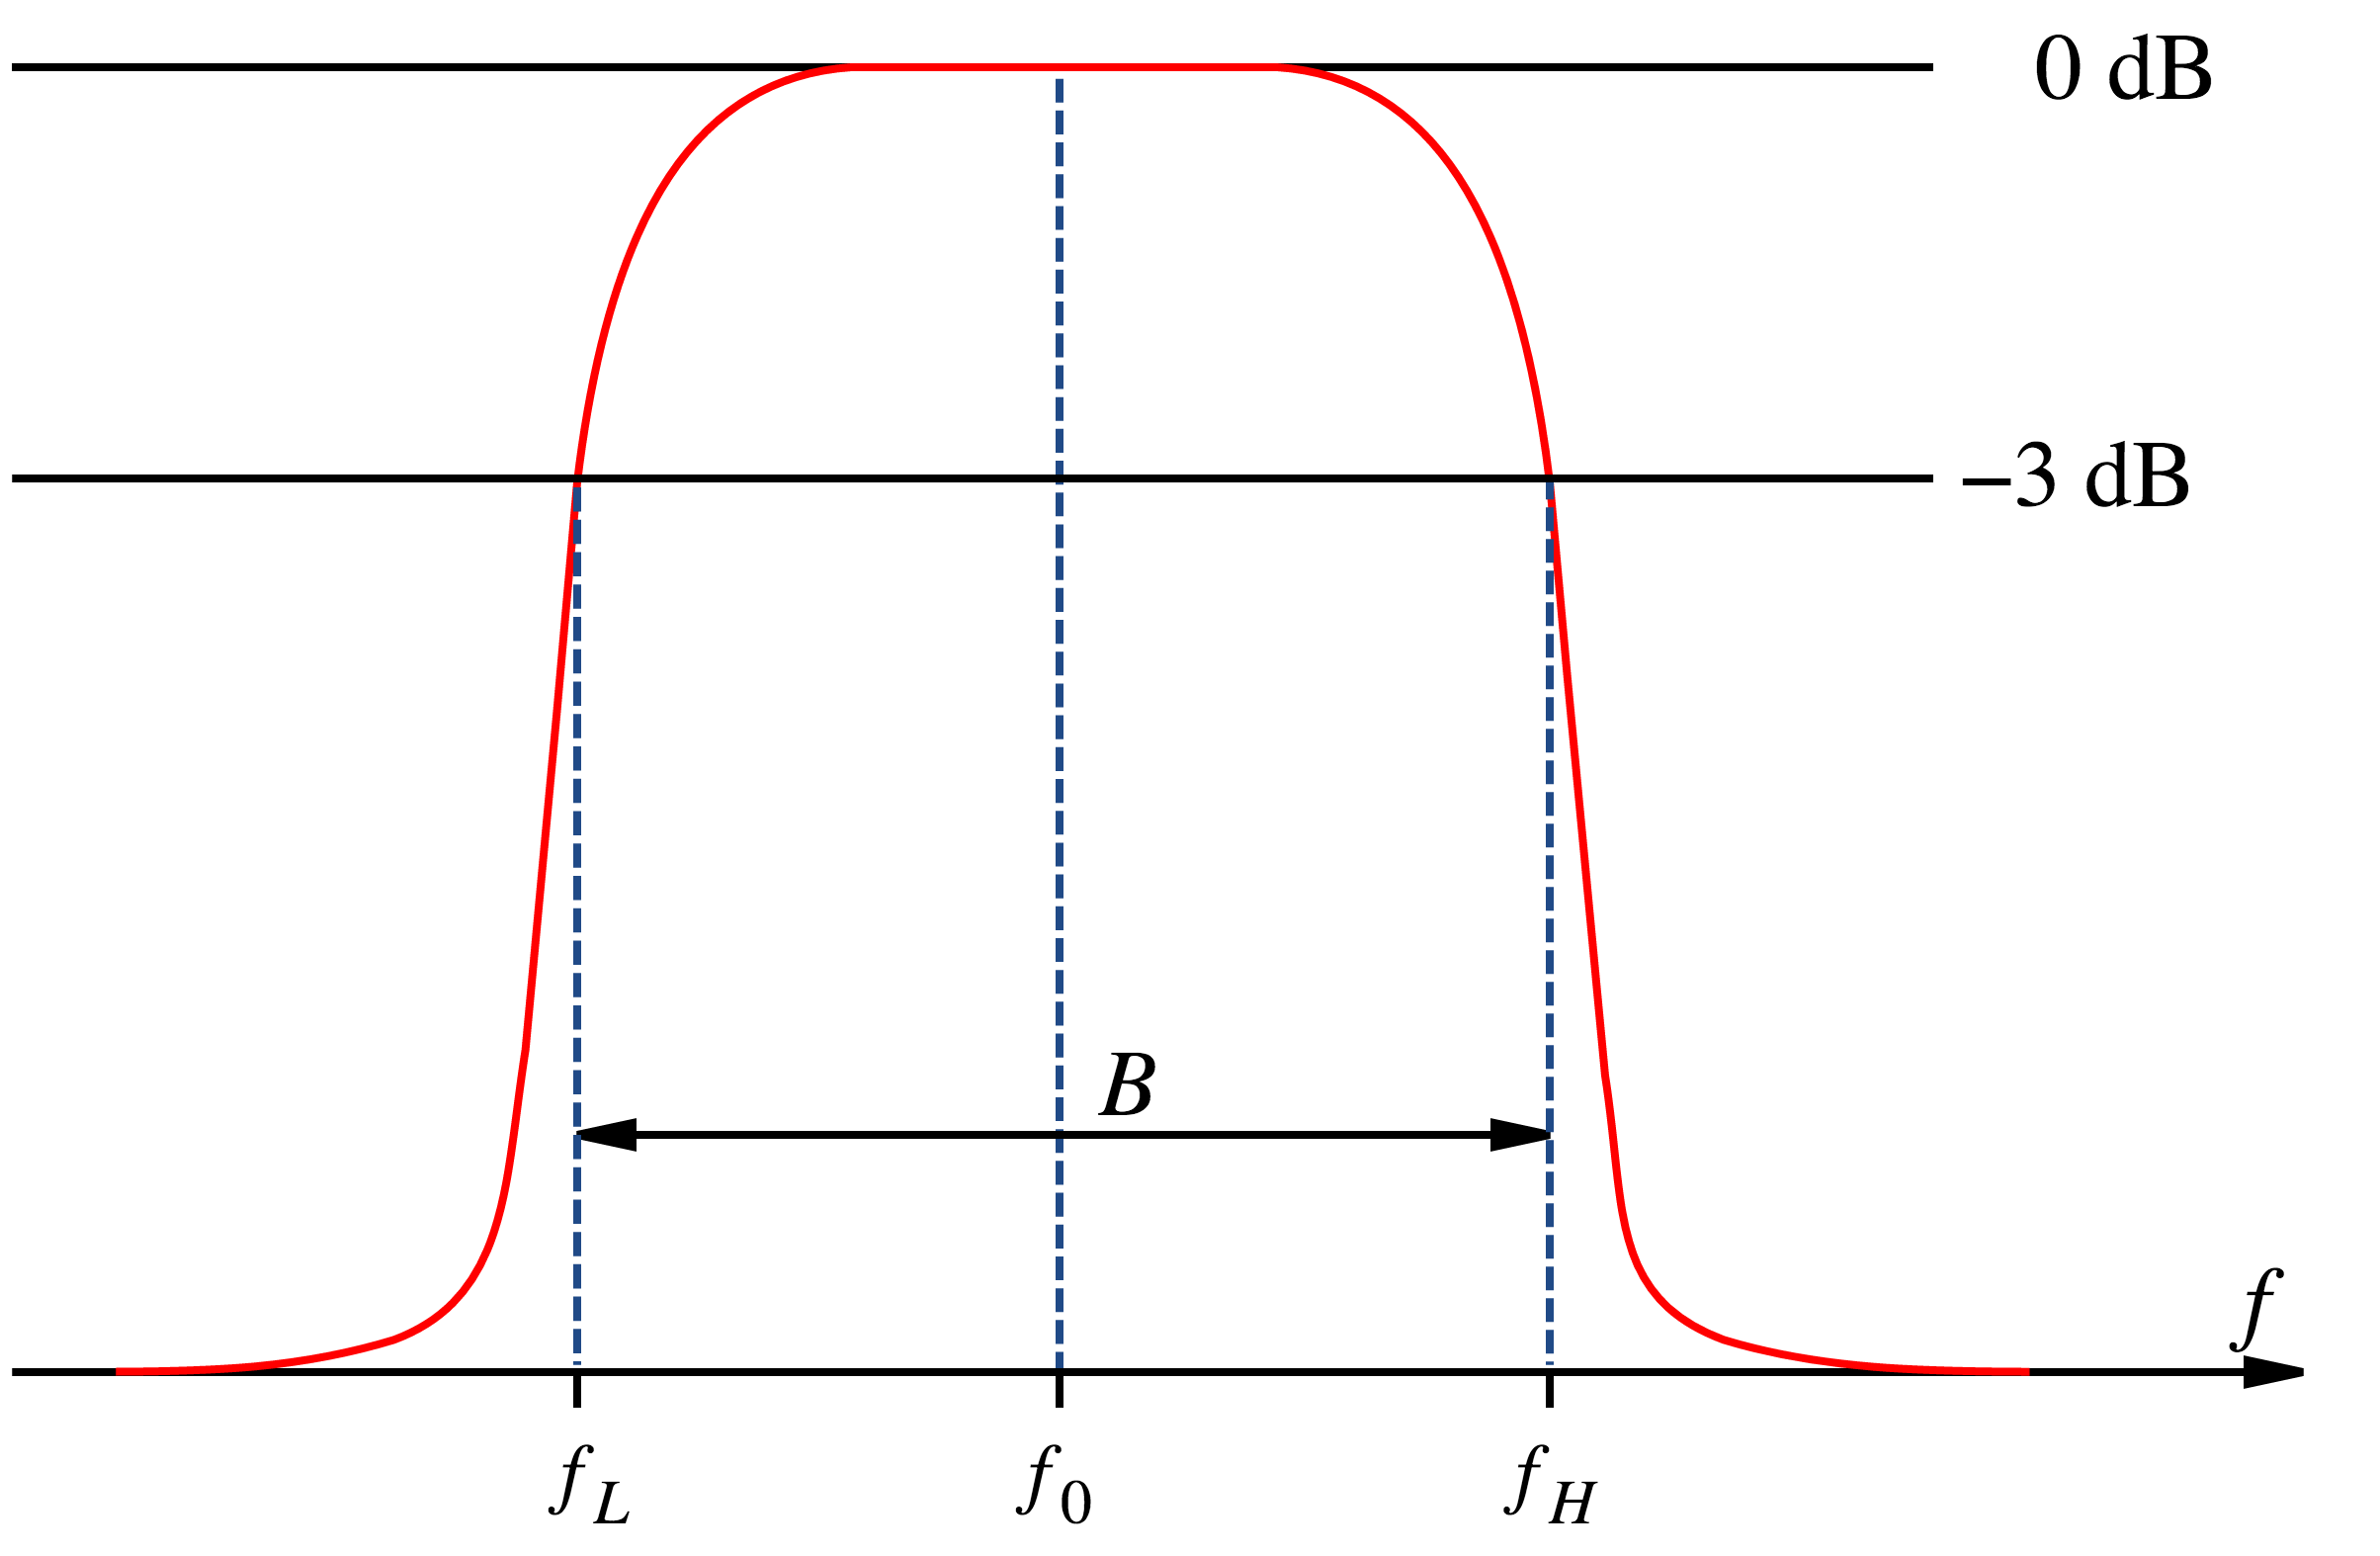
\includegraphics[width=\textwidth]{graphics/bandpassbode}
		\caption{The frequency response of a bandpass filter with lower 3dB frequency $f_L$ and upper 3dB frequency $f_H$~\cite{bandpass}.}
		\label{fig:bandpass}
	\end{figure}
	
	
	
	
	
	
	
	
	
	
	
	
	
	
	\pagebreak
	\section{Progress with my project}
	
	\subsection{Last week}
	This week I worked mostly on software design and distinguished more between each of the modules I need for my project. This is important for me because a complicated project like this needs to be well organized so that I can work systematically on each module and it helps me keep my sanity. The result is displayed in figure~\ref{fig:software}.
	
	With this design, I worked on the IMU module which uses an SPI module (not shown in figure~\ref{fig:software}) to communicate with the sensor itself. This is now in it's final stages before I can start implementing other parts of the robot that use the actual IMU sensor values.
	
	\begin{figure}[h]
		\centering
		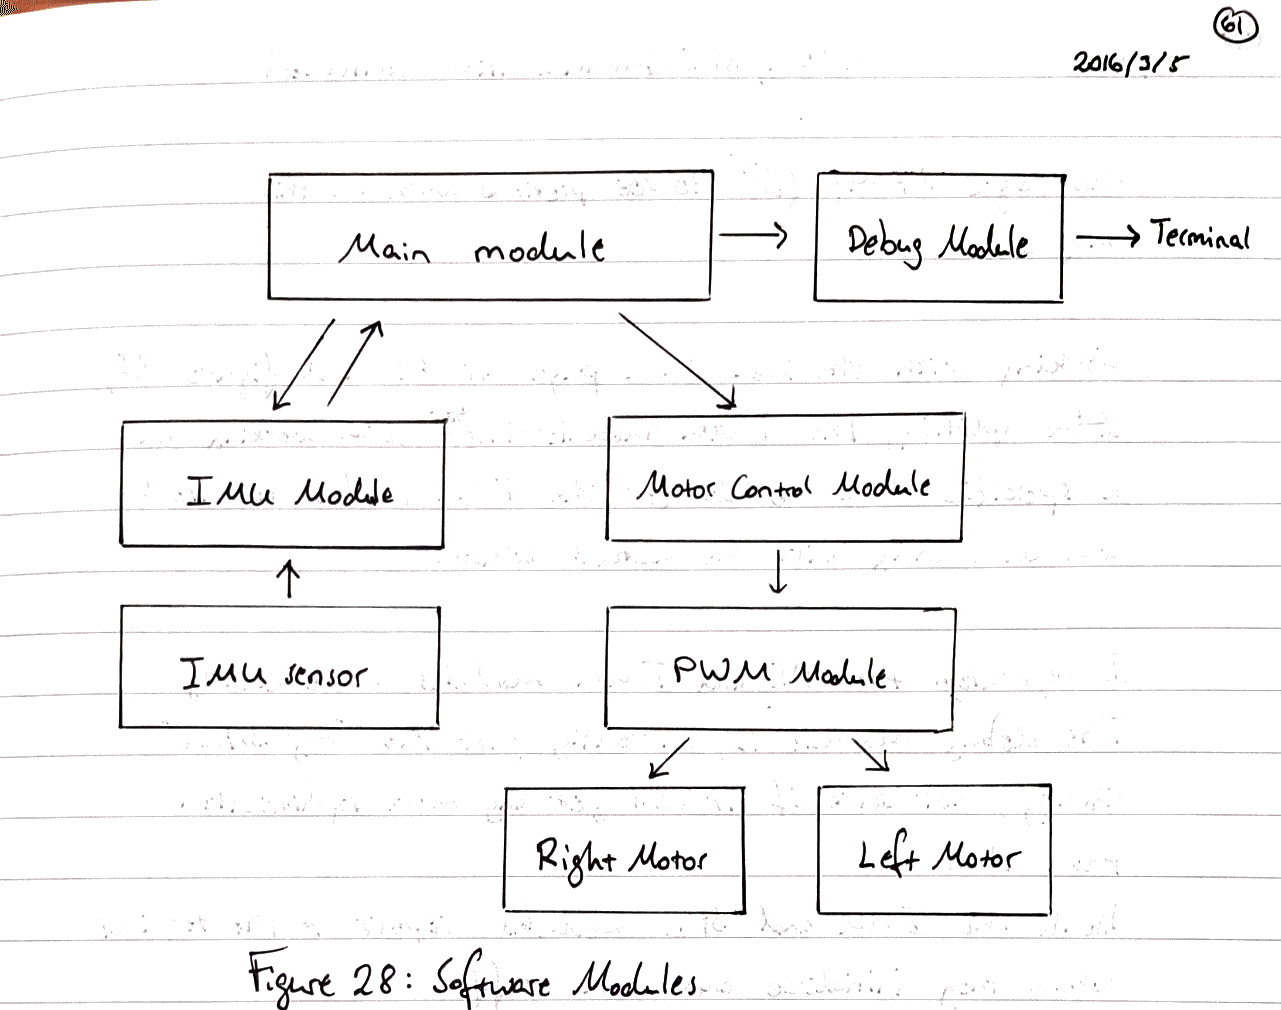
\includegraphics[width=0.8\textwidth]{graphics/software}
		\caption{Breakdown of the software modules needed for the inverted pendulum project}
		\label{fig:software}
	\end{figure}
	
	After discussion with my peers, I have decided to implement the PWM module using the output compare pins that can be toggled using interrupts. That way the PWM functionality is reduced in complexity from the main programs point of view.
	
	\pagebreak
	\subsection{Next week}
	
	\begin{table}[h]
		\centering
		\begin{tabular}{llc}
			\toprule
			Task no.	&	Task	&	ETC\footnotemark\\
			\midrule
			1	&	\begin{tabular}{@{}l@{}}Finish the IMU module\\\end{tabular} &	5 hours \\	
			\midrule	
			2	&	\begin{tabular}{@{}l@{}}Write the PWM code that uses output compare pins\end{tabular}	&	10 hours\\
			\midrule
			3	&	\begin{tabular}{@{}l@{}}Test the accuracy of the\\IMU sensor\end{tabular}	&	5 hours\\
			\midrule
			4	&		\begin{tabular}{@{}l@{}}Plan the control system and\\start designing at a high level\end{tabular}	&	5 hours\\
			\bottomrule
		\end{tabular}
		\label{tab:nextweek}
	\end{table}
	
	
	\footnotetext{Estimated Time to Complete}

	\subsection{Long term plan}
	
	\begin{table}[h]
		\centering
		\hspace*{-2cm}
		\begin{tabular}{lccc}
			\toprule
			Week	&	Software design	&	Mechanical design	&	Testing\\
			\midrule
			9	&	IMU \& PWM	&	\begin{tabular}{@{}l@{}}Power circuitry\\2nd prototype\end{tabular}	&	\begin{tabular}{@{}l@{}}Estimate power consumption\\PID motor control\end{tabular}\\
			\midrule
			10	&	Rethink PID control	&	3D drawing of the robot	&	Power consumption	\\
			\midrule
			11	&	\begin{tabular}{@{}l@{}}Integrate IMU, PID\\ and PWM modules\end{tabular}	&	Altium schematics of electronics	&	Integration\\
			\midrule
			12	&	Integration	&	Integration	&	Integration	\\
			\bottomrule
		\end{tabular}
		\label{tab:longterm}
		\hspace*{-2cm}
	\end{table}
	
	
	
\pagebreak
%\section*{Appendices}
\appendix



\pagebreak
\printbibliography

\end{document}